\documentclass{standalone}
\usepackage{tikz}
\usetikzlibrary{patterns, positioning}
\usepackage[sfdefault]{ClearSans} %% option 'sfdefault' activates Clear Sans as the default text font
\usepackage[T1]{fontenc}

\begin{document}
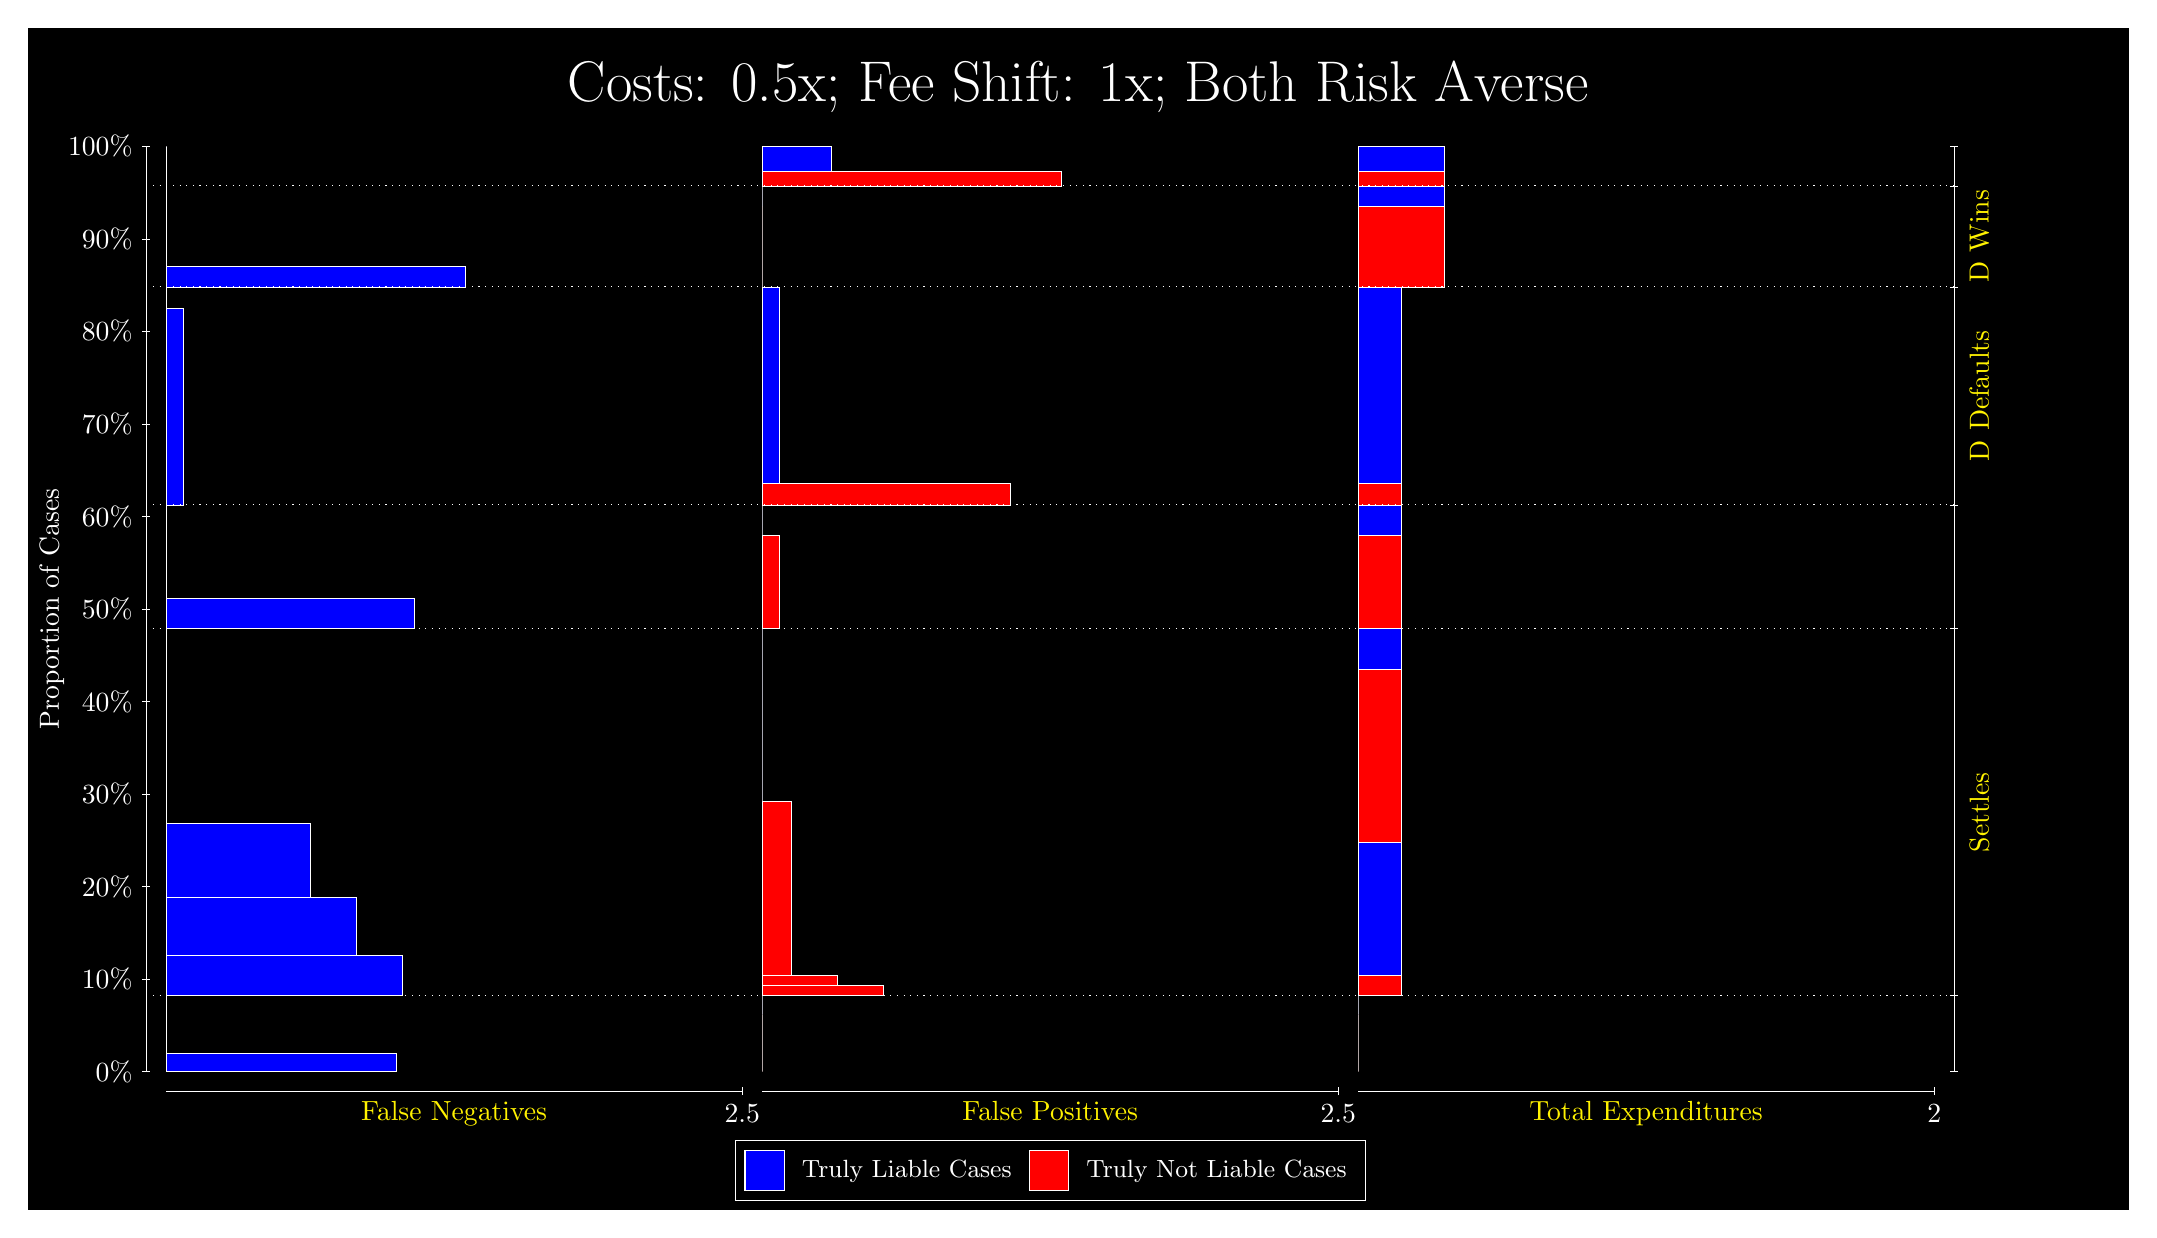
\begin{tikzpicture}
\draw[fill=black] (0,0) rectangle (26.667,15);
\draw[text=white] (0,13.5) rectangle (26.667,15) node[midway] {\huge Costs: 0.5x; Fee Shift: 1x; Both Risk Averse};
\draw[white, very thin] (1.5,1.75) -- (1.5,13.5);
\node[rotate=90, text=white, anchor=center] at (0.3, 7.625) {Proportion of Cases};
\draw[white, very thin] (1.45,1.75) -- (1.55,1.75);
\node[text=white, anchor=east] at (1.45, 1.75) {0\%};
\draw[white, very thin] (1.45,2.925) -- (1.55,2.925);
\node[text=white, anchor=east] at (1.45, 2.925) {10\%};
\draw[white, very thin] (1.45,4.1) -- (1.55,4.1);
\node[text=white, anchor=east] at (1.45, 4.1) {20\%};
\draw[white, very thin] (1.45,5.275) -- (1.55,5.275);
\node[text=white, anchor=east] at (1.45, 5.275) {30\%};
\draw[white, very thin] (1.45,6.45) -- (1.55,6.45);
\node[text=white, anchor=east] at (1.45, 6.45) {40\%};
\draw[white, very thin] (1.45,7.625) -- (1.55,7.625);
\node[text=white, anchor=east] at (1.45, 7.625) {50\%};
\draw[white, very thin] (1.45,8.8) -- (1.55,8.8);
\node[text=white, anchor=east] at (1.45, 8.8) {60\%};
\draw[white, very thin] (1.45,9.975) -- (1.55,9.975);
\node[text=white, anchor=east] at (1.45, 9.975) {70\%};
\draw[white, very thin] (1.45,11.15) -- (1.55,11.15);
\node[text=white, anchor=east] at (1.45, 11.15) {80\%};
\draw[white, very thin] (1.45,12.325) -- (1.55,12.325);
\node[text=white, anchor=east] at (1.45, 12.325) {90\%};
\draw[white, very thin] (1.45,13.5) -- (1.55,13.5);
\node[text=white, anchor=east] at (1.45, 13.5) {100\%};

\draw[white, very thin] (24.457,1.75) -- (24.457,13.5);
\draw[white, very thin] (24.407,1.75) -- (24.507,1.75);
\node[anchor=west] at (24.407, 1.75) {};
\draw[white, very thin] (24.407,2.7137) -- (24.507,2.7137);
\node[anchor=west] at (24.407, 2.7137) {};
\draw[white, very thin] (24.407,7.3736) -- (24.507,7.3736);
\node[anchor=west] at (24.407, 7.3736) {};
\draw[white, very thin] (24.407,8.947) -- (24.507,8.947);
\node[anchor=west] at (24.407, 8.947) {};
\draw[white, very thin] (24.407,11.716) -- (24.507,11.716);
\node[anchor=west] at (24.407, 11.716) {};
\draw[white, very thin] (24.407,12.997) -- (24.507,12.997);
\node[anchor=west] at (24.407, 12.997) {};
\draw[white, very thin] (24.407,13.5) -- (24.507,13.5);
\node[anchor=west] at (24.407, 13.5) {};

\draw[white, very thin, fill=blue] (1.75,1.75) rectangle (4.6775,1.9863);
\draw[white, very thin, fill=red] (1.75,1.9863) rectangle (1.75,2.7137);
\draw[white, very thin, fill=blue] (1.75,2.7137) rectangle (4.7507,3.2224);
\draw[white, very thin, fill=blue] (1.75,3.2224) rectangle (4.1652,3.9691);
\draw[white, very thin, fill=blue] (1.75,3.9691) rectangle (3.5797,4.9061);
\draw[white, very thin, fill=red] (1.75,4.9061) rectangle (1.75,7.3736);
\draw[white, very thin, fill=blue] (1.75,7.3736) rectangle (4.8971,7.7587);
\draw[white, very thin, fill=red] (1.75,7.7587) rectangle (1.75,8.947);
\draw[white, very thin, fill=blue] (1.75,8.947) rectangle (1.9696,11.437);
\draw[white, very thin, fill=red] (1.75,11.437) rectangle (1.75,11.716);
\draw[white, very thin, fill=blue] (1.75,11.716) rectangle (5.5558,11.974);
\draw[white, very thin, fill=red] (1.75,11.974) rectangle (1.75,12.997);
\draw[white, very thin, fill=red] (1.75,12.997) rectangle (1.75,13.187);
\draw[white, very thin, fill=blue] (1.75,13.187) rectangle (1.75,13.5);
\draw[white, very thin, fill=red] (9.3189,1.75) rectangle (9.3189,2.4774);
\draw[white, very thin, fill=blue] (9.3189,2.4774) rectangle (9.3189,2.7137);
\draw[white, very thin, fill=red] (9.3189,2.7137) rectangle (10.856,2.8476);
\draw[white, very thin, fill=red] (9.3189,2.8476) rectangle (10.27,2.978);
\draw[white, very thin, fill=red] (9.3189,2.978) rectangle (9.6848,5.1812);
\draw[white, very thin, fill=blue] (9.3189,5.1812) rectangle (9.3189,7.3736);
\draw[white, very thin, fill=red] (9.3189,7.3736) rectangle (9.5384,8.5619);
\draw[white, very thin, fill=blue] (9.3189,8.5619) rectangle (9.3189,8.947);
\draw[white, very thin, fill=red] (9.3189,8.947) rectangle (12.466,9.2257);
\draw[white, very thin, fill=blue] (9.3189,9.2257) rectangle (9.5384,11.716);
\draw[white, very thin, fill=red] (9.3189,11.716) rectangle (9.3189,12.739);
\draw[white, very thin, fill=blue] (9.3189,12.739) rectangle (9.3189,12.997);
\draw[white, very thin, fill=red] (9.3189,12.997) rectangle (13.125,13.187);
\draw[white, very thin, fill=blue] (9.3189,13.187) rectangle (10.197,13.5);
\draw[white, very thin, fill=red] (16.888,1.75) rectangle (16.888,2.4774);
\draw[white, very thin, fill=blue] (16.888,2.4774) rectangle (16.888,2.7137);
\draw[white, very thin, fill=red] (16.888,2.7137) rectangle (17.437,2.978);
\draw[white, very thin, fill=blue] (16.888,2.978) rectangle (17.437,4.6617);
\draw[white, very thin, fill=red] (16.888,4.6617) rectangle (17.437,6.8649);
\draw[white, very thin, fill=blue] (16.888,6.8649) rectangle (17.437,7.3736);
\draw[white, very thin, fill=red] (16.888,7.3736) rectangle (17.437,8.5619);
\draw[white, very thin, fill=blue] (16.888,8.5619) rectangle (17.437,8.947);
\draw[white, very thin, fill=red] (16.888,8.947) rectangle (17.437,9.2257);
\draw[white, very thin, fill=blue] (16.888,9.2257) rectangle (17.437,11.716);
\draw[white, very thin, fill=red] (16.888,11.716) rectangle (17.986,12.739);
\draw[white, very thin, fill=blue] (16.888,12.739) rectangle (17.986,12.997);
\draw[white, very thin, fill=red] (16.888,12.997) rectangle (17.986,13.187);
\draw[white, very thin, fill=blue] (16.888,13.187) rectangle (17.986,13.5);
\draw[white, dotted] (1.5,2.7137) -- (24.457,2.7137);
\draw[white, dotted] (1.5,7.3736) -- (24.457,7.3736);
\draw[white, dotted] (1.5,8.947) -- (24.457,8.947);
\draw[white, dotted] (1.5,11.716) -- (24.457,11.716);
\draw[white, dotted] (1.5,12.997) -- (24.457,12.997);
\draw[white, very thin] (1.75,1.5) -- (9.0689,1.5);
\node[text=yellow, anchor=north] at (5.4094, 1.5) {False Negatives};
\draw[white, very thin] (9.0689,1.45) -- (9.0689,1.55);
\node[text=white, anchor=north] at (9.0689, 1.45) {2.5};

\draw[white, very thin] (9.3189,1.5) -- (16.638,1.5);
\node[text=yellow, anchor=north] at (12.978, 1.5) {False Positives};
\draw[white, very thin] (16.638,1.45) -- (16.638,1.55);
\node[text=white, anchor=north] at (16.638, 1.45) {2.5};

\draw[white, very thin] (16.888,1.5) -- (24.207,1.5);
\node[text=yellow, anchor=north] at (20.547, 1.5) {Total Expenditures};
\draw[white, very thin] (24.207,1.45) -- (24.207,1.55);
\node[text=white, anchor=north] at (24.207, 1.45) {2};


\node[text=yellow, centered, rotate=90] at (24.777, 5.0437) {Settles};

\node[text=yellow, centered, rotate=90] at (24.777, 10.331) {D Defaults};
\node[text=yellow, centered, rotate=90] at (24.777, 12.357) {D Wins};


\draw (12.978300999999998,1.5) node[draw=none] (baseCoordinate) {};
\begin{scope}[align=center]
        \matrix[scale=0.5, draw=white, below=0.5cm of baseCoordinate, nodes={draw}, column sep=0.1cm]{
            \node[rectangle, draw, minimum width=0.5cm, minimum height=0.5cm, fill=blue] {}; &
            \node[draw=none, font=\small, text=white] (B) {Truly Liable Cases}; &
            \node[rectangle, draw, minimum width=0.5cm, minimum height=0.5cm, fill=red] {}; &
            \node[draw=none, font=\small, text=white] (B) {Truly Not Liable Cases}; \\
            };
\end{scope}

\end{tikzpicture}
\end{document}